\documentclass[conference]{IEEEtran}
\IEEEoverridecommandlockouts
% The preceding line is only needed to identify funding in the first footnote. If that is unneeded, please comment it out.
\usepackage{cite}
\usepackage{amsmath,amssymb,amsfonts}
\usepackage{algorithmic}
\usepackage{textcomp}
\usepackage{xcolor}
\usepackage{graphicx}
\usepackage{subfigure}
\def\BibTeX{{\rm B\kern-.05em{\sc i\kern-.025em b}\kern-.08em
    T\kern-.1667em\lower.7ex\hbox{E}\kern-.125emX}}
\begin{document}

\title{A Load-adaptive CSMA MAC Protocol for Mobile Underwater Acoustic Sensor Networks\\
}

\author{\IEEEauthorblockN{1\textsuperscript{st} Given Name Surname}
\IEEEauthorblockA{\textit{dept. name of organization (of Aff.)} \\
\textit{name of organization (of Aff.)}\\
City, Country \\
email address}
\and
\IEEEauthorblockN{2\textsuperscript{nd} Given Name Surname}
\IEEEauthorblockA{\textit{dept. name of organization (of Aff.)} \\
\textit{name of organization (of Aff.)}\\
City, Country \\
email address}
\and
\IEEEauthorblockN{3\textsuperscript{rd} Given Name Surname}
\IEEEauthorblockA{\textit{dept. name of organization (of Aff.)} \\
\textit{name of organization (of Aff.)}\\
City, Country \\
email address}
}

\maketitle

\begin{abstract}
Autonomous underwater vehicles (AUVs) and unmanned underwater vehicles (UUVs) have been applied in underwater acoustic sensor networks to collect data. Consider a single-hop communication occasion where mobile nodes tour around the area of pre-deployed static nodes and gather data generated at static nodes. On this occasion, a load adaptive CSMA/CA MAC protocol for mobile underwater acoustic network (LACC-M) is proposed. The protocol adopts two transmission modes to satisfy different requirements of different network loads. Broadcast (BCT) frame is specially designed to allow mobile nodes joining and exiting the network, and changing the transmission mode depending on the network load. Given an overall consideration of throughput, end-to-end delay, successful delivery rate and energy consumption, simulations show that LACC-M outperforms other two contention-based protocols, SFAMA and UWALOHA in specific application scenarios.
\end{abstract}

\begin{IEEEkeywords}
underwater acoustic sensor network, media access control, contention-based protocol, mobile node access, load adaptive
\end{IEEEkeywords}

\section{Introduction}
Mobile underwater acoustic sensor networks (UWASNs) have been proposed as a way to collect, store, and retrieve data
in seafloor observation\cite{vasilescu2005data}. Mobile nodes like UUVs/AUVs can expand the observation area, and detect node failure of the static underwater network. While static nodes can navigate mobile nodes with information of locations and surroundings. Accordingly, mobile underwater acoustic sensor networks become increasingly attractive in underwater networking technology\cite{cui2006challenges}. However, characteristics of underwater acoustic channel along with the dynamic nature of network topology poses challenges to mobile underwater networking. 

Noh et al. propose a contention-based protocol called delay-aware opportunistic transmission scheduling (DOTS) protocol in\cite{noh2014dots} for mobile UWASNs. It uses passively obtained local information to increase the chances of concurrent
transmissions while reducing the likelihood of collisions. 

In\cite{Zhang2016Dynamic}, dynamic node cooperation is proposed for data collection network. If single-hop transmission fails in th first round, one node can be selected as a relay to  transmit the data in the second phase. The relay nodes participating the cooperation are selected by the destination based on the channel quality.
% However, the forward phase will increase the load and energy consumption as well.

In\cite{mao2016ltm}, a location-based TDMA MAC(LTM-MAC) is proposed to minimum accessing time of AUV and waiting time of static nodes if no AUVs intend to transmit. Dynamic programming is adopted to obtain a solution for the optimum order. 

Reference \cite{deng2017hybrid} assumes that a hybrid protocol is more suitable for the data collection network in mobile UWASNs rather then a unified single-mode protocol. The traffic load in
each layer is different. Accordingly, a contention-based MAC protocol is performed in the lightly loaded sub-network, and a reservation-based MAC protocol is carried out in the heavily loaded sub-network.
 
In this paper, we propose a load adaptive CSMA/CA MAC for mobile UWASNs, LACC-M. In LACC-M, mobile nodes can instantly join and exit the network by introducing the broadcast (BCT) frame. The BCT frame also takes the responsibility to inform static nodes of the current state of network load. Hence, different transmission flows can be employed in different network states.

The rest of this paper is organized as follows. Section II describes the algorithm of LACC-M in detail. Section III analyzes the performance of the protocol in theory. Section IV conducts simulations and evaluates the performance compared to contention-based MAC protocols, UWALOHA and slotted FAMA (SFAMA). Conclusion and future work are presented at the end of the paper.

\section{LACC-M PROTOCOL DESIGN}

In this section, the protocol model is introduced. Contention-based carrier sense multiple access/collision avoidance (CSMA/CA) mechanism lays the foundation of the protocol. On this basis, BCT frame is designed especially for the mobile nodes to collect data from static nodes. It's also worth mention that data transmission flow is adaptive to the network load in time.

\subsection{basic mechanism: CSMA/CA}

Assuming that underwater nodes can overhear the transmission of the others, CSMA/CA is applied to maximum the usage of the channel. The detailed flow is illustrated in \ref{f1}. 
\begin{figure}[ht]
	\centerline{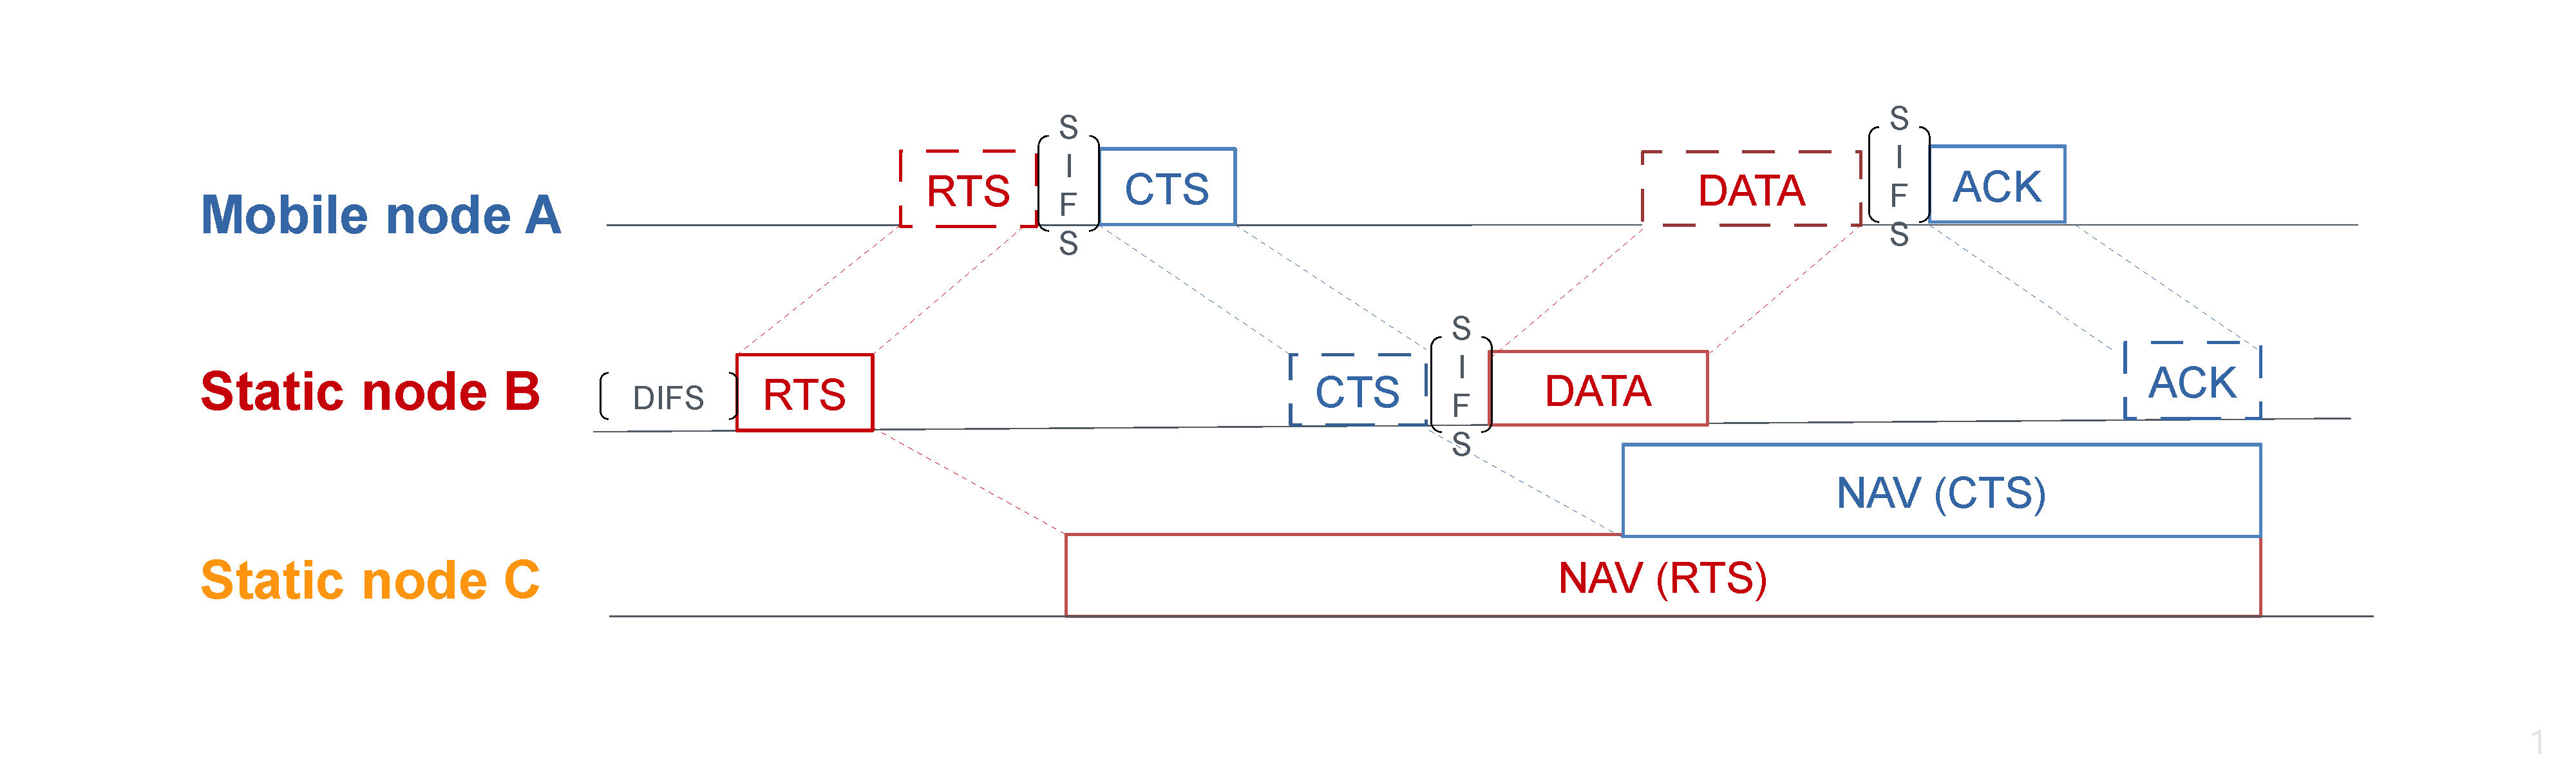
\includegraphics[scale=0.12]{figures/1.pdf}}
	\caption{Illustration of CSMA/CA}
	\label{f1}
\end{figure}
Before each sending, the node will listen to the channel for a set time such as Short Interframe Space (SIFS), determined by 
\begin{equation*}
\begin{aligned}
SIFSTime=&ReceiveDelay+MACProcessingDelay\\&+RxTxTurnaroundTime
\end{aligned}
\end{equation*} 
and DCF Interframe Space (DIFS),determined by. 
\begin{equation*}
DIFS=SIFS+(2*SlotTime)
\end{equation*}
SlotTime is decided by physical channel, mostly up to length of propagation delay and MAC processing delay.

Collision avoidance is realized by network allocation vector (NAV). Once node C receives RTS frame from node A or CTS frame from node B, whose destination is different from node C, node C will backoff for corresponding NAV time recorded in the frame. We make reference to \cite{cho2016network} to optimize NAV. Specific settings are illustrated in section IV.

\subsection{introduction of BCT frame}
Broadcast (BCT) frame is introduced for the instant joining and exiting of mobile nodes, and takes responsibility to inform static nodes of the current state of network load at the same time.

The mobile nodes will send BCT frame to neighboring nodes at intervals of a set length $T_{interval}$. Static nodes receive the frame and send data stream to mobile nodes if needed. Static nodes will stop the transmission if none of BCT frame is received in time of $2T_{interval}$ since last BCT frame.

The sending and receiving of BCT frame don't affect the ongoing data interaction. The whole stage in which a mobile node joins and then exits the network is illustrated in fig.\ref{ml}.
\begin{figure}[ht]
	\centerline{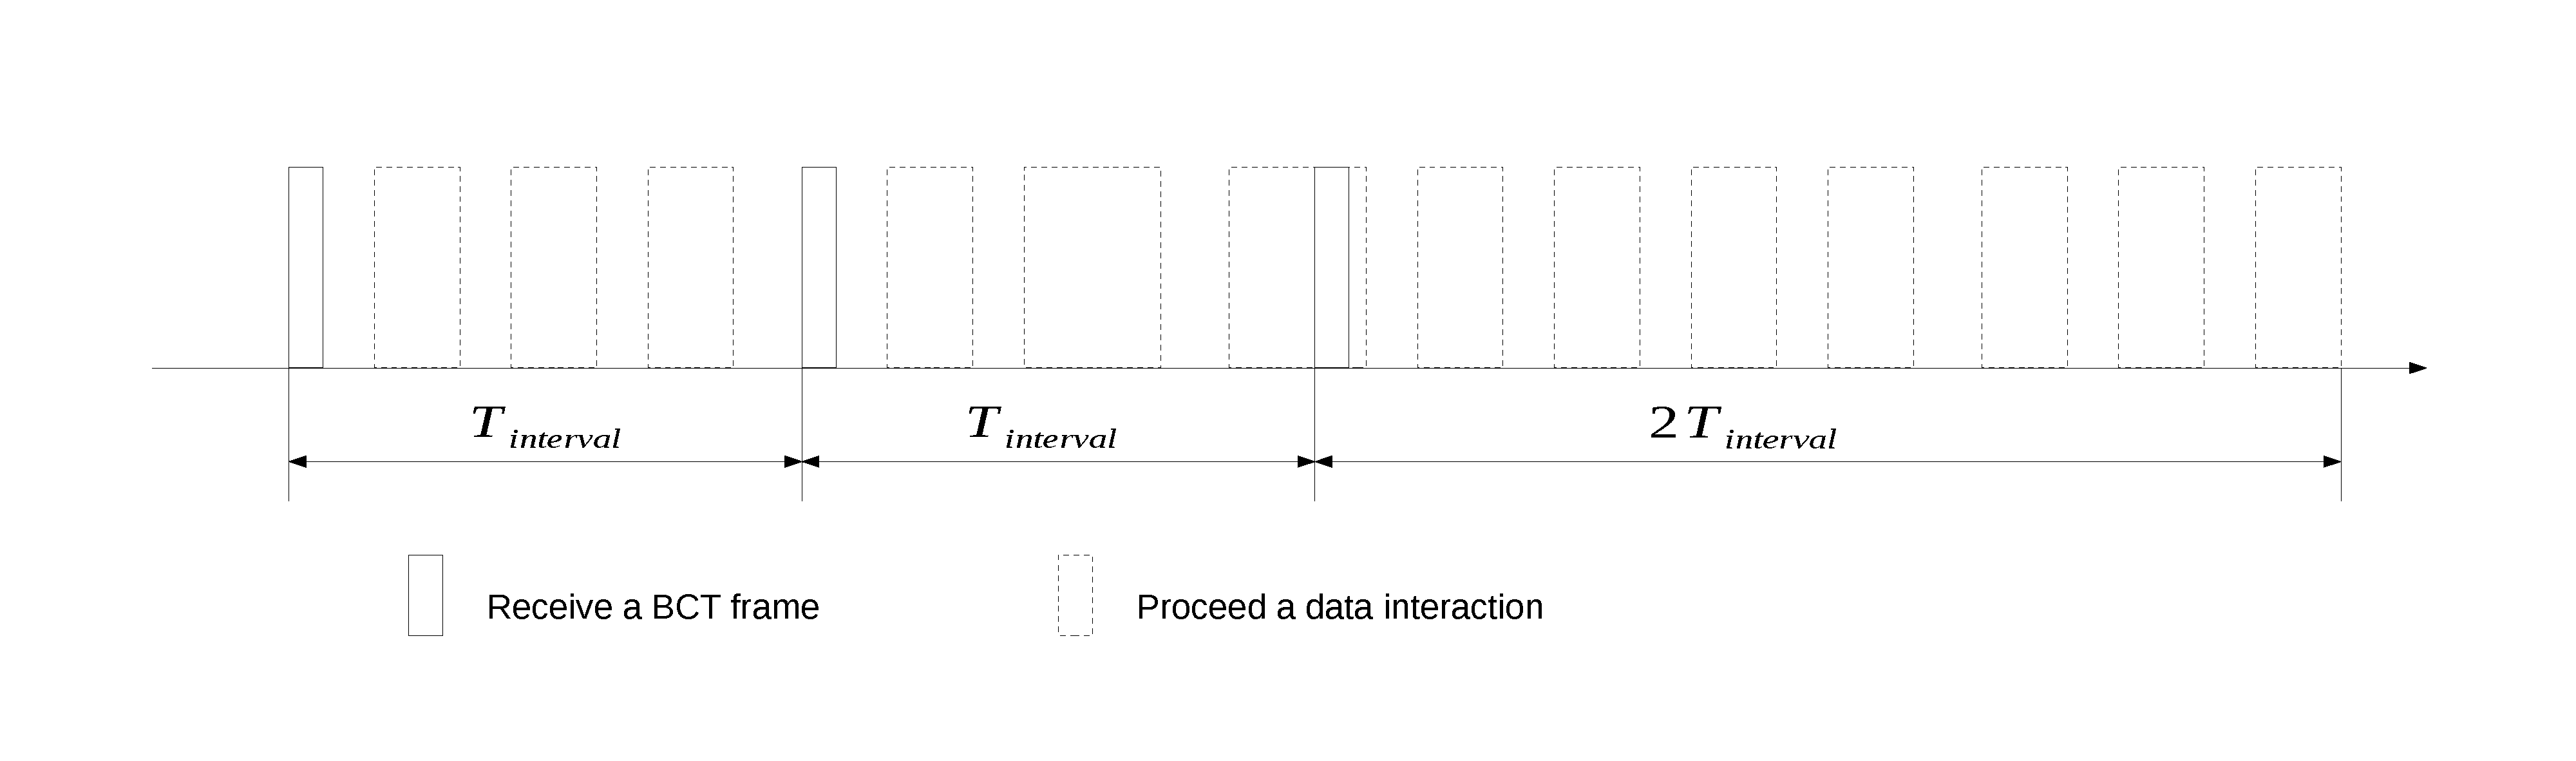
\includegraphics[scale=0.15]{figures/3.pdf}}
	\caption{The transmission period of static nodes}
	\label{ml}
\end{figure}

\subsection{load-adaptive transmission mchanism}
The BCT frame also plays an important role in load-adaptive data transmission mchanism. The load state of the network is classified into 2 modes, `high' and `low'. The data transmission mechanism, high-load mode or low-load mode, will be applied in corresponding load state. The flag bit of the load state is added in the BCT frame thus mobile nodes are able to change the transmission mode of neighboring static nodes.

In the low-load mode, the transmission flow is the same as fig.\ref{f1}. While in the high-load mode, two data frames will be transmitted after one handshaking as fig.\ref{ll} shows. The interframe space between two data frames chooses SIFS, the minimum space which gives the following frame highest priority. The deferring time, NAV, needs to be extended to make room for one more data frame and a SIFS time. 
\begin{figure}[ht]
	\centerline{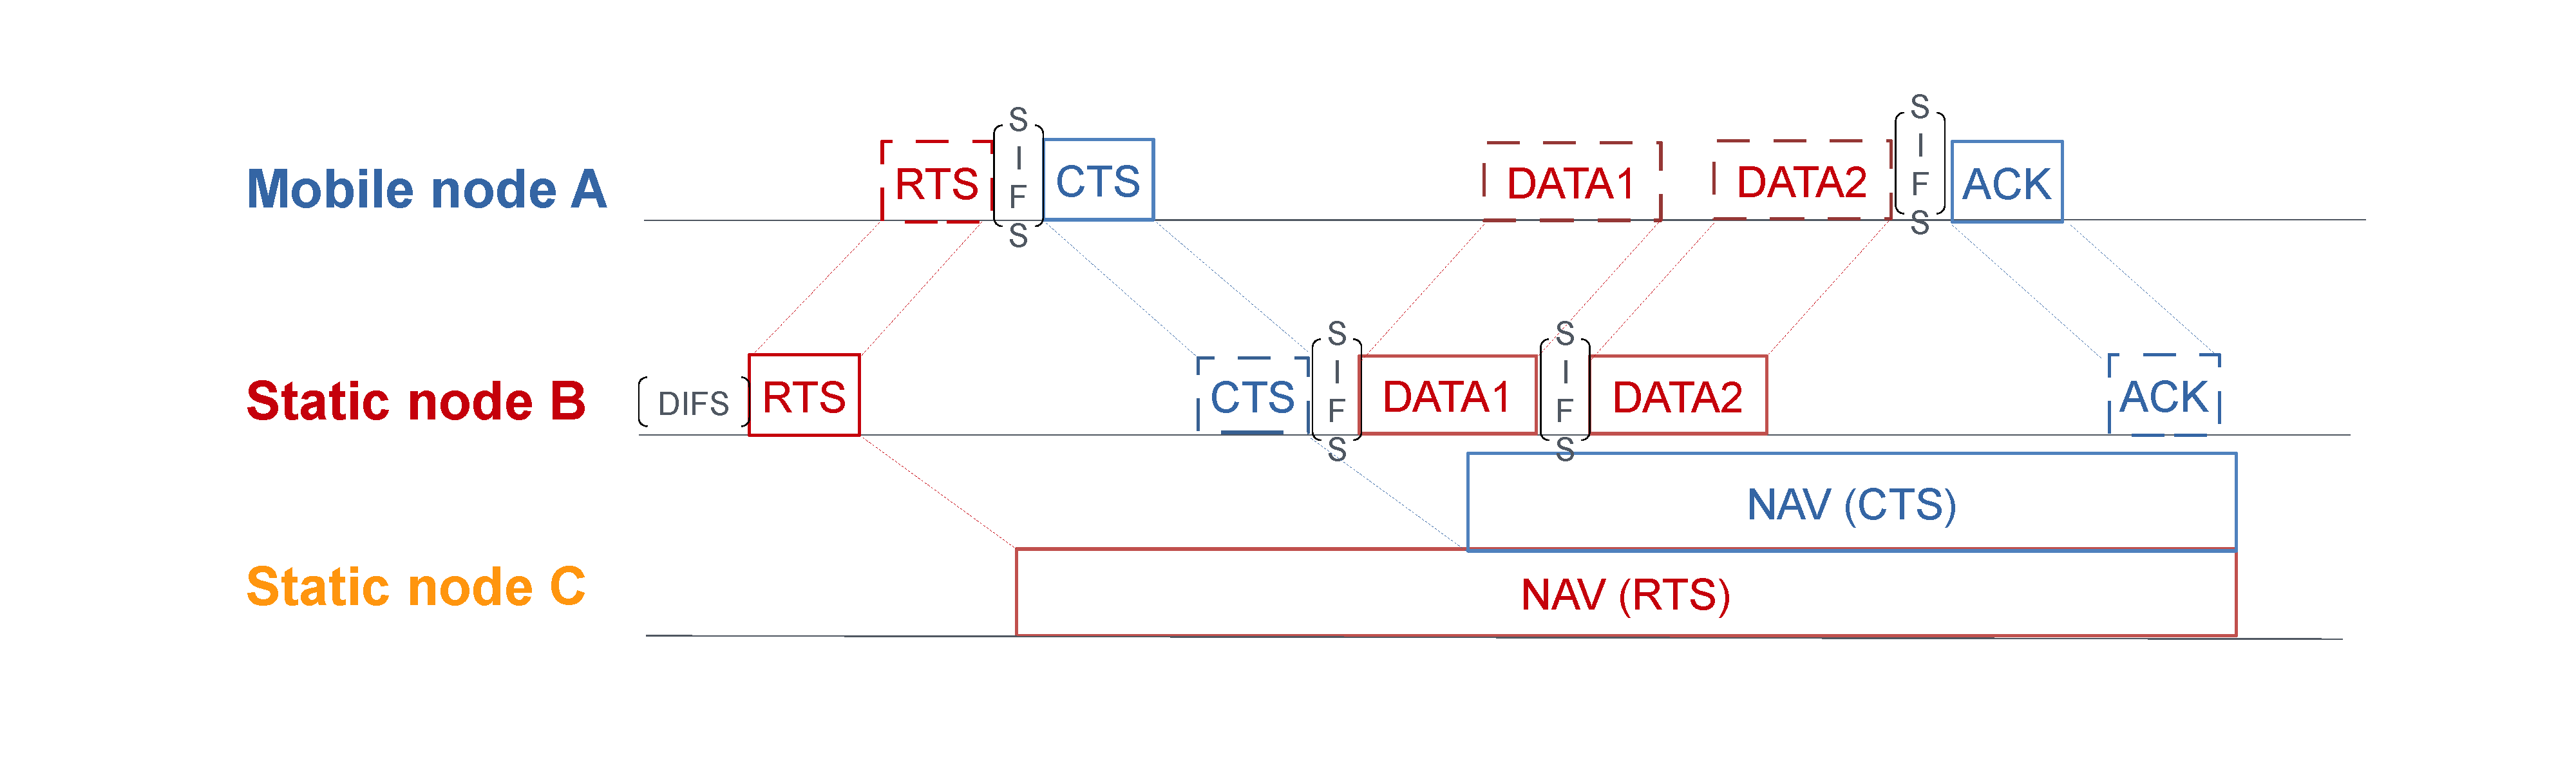
\includegraphics[scale=0.12]{figures/2.pdf}}
	\caption{transmission flow in high-load mode}
	\label{ll}
\end{figure}


Nodes will be allocated into five states in the data interaction. They are RTS, CTS, ACK, IDLE and SEND state. When node A starts sending RTS frame, the state of itself is set into RTS. Node A will change the state into IDLE only if it received CTS frame or the configured timeout occurred. Similarly, sending CTS frame corresponds to CTS state, ACK frame to ACK state, BCT/DATA frame to SEND state. Receiving expected frame and configured timeout both cause the change of the state and promote the transmission flow.

It's noteworthy that, in the high-load transmission mode, timeouts set for the two data frames are different. For the first data frame, the SEND state can only be changed after a transmitting time of one frame. For the second frame, timeout equals
\begin{equation*}
\begin{aligned}
T_{timeout}=&txtime(DATA)+SIFS+txtime(ACK)\\&+MaxPropagationDelay
\end{aligned}
\end{equation*}


\section{performance analysis}
Based on the flow model\cite{kleinrock1975packet}, the normalized throughput can be calculated as
\begin{equation}
S=\frac{\overline U}{\overline B+\overline I}
\label{11}
\end{equation}

$\overline U$ denotes expected time for transmitting useful data, $\overline B$ denotes expected time when node is busy, $\overline I$ denotes expected time when node is idle. 

\subsection {low-load transmission mode}
In LACC-M protocol,there are two circumstances where collisions will happen. The first one is caused by RTS frames sent by hidden terminals. As shown in fig.\ref{fig:example}, mobile node 2 is in the communication range of static node 1 and static node 3. Node 3, out of range of node 1, is node 1's hidden terminal. When node 1 interacts with node 2, the RTS frame caused by node 3 will influence node 2's receiving of node 1's RTS frame or DATA frame. The second circumstance is caused by the BCT frames sent periodically by mobile nodes. Mobile nodes other than node 2 send BCT frames periodically, which may cause collisions if node 1 is receiving CTS or ACK frame from node 2.
\begin{figure}[!ht]
	\centering
	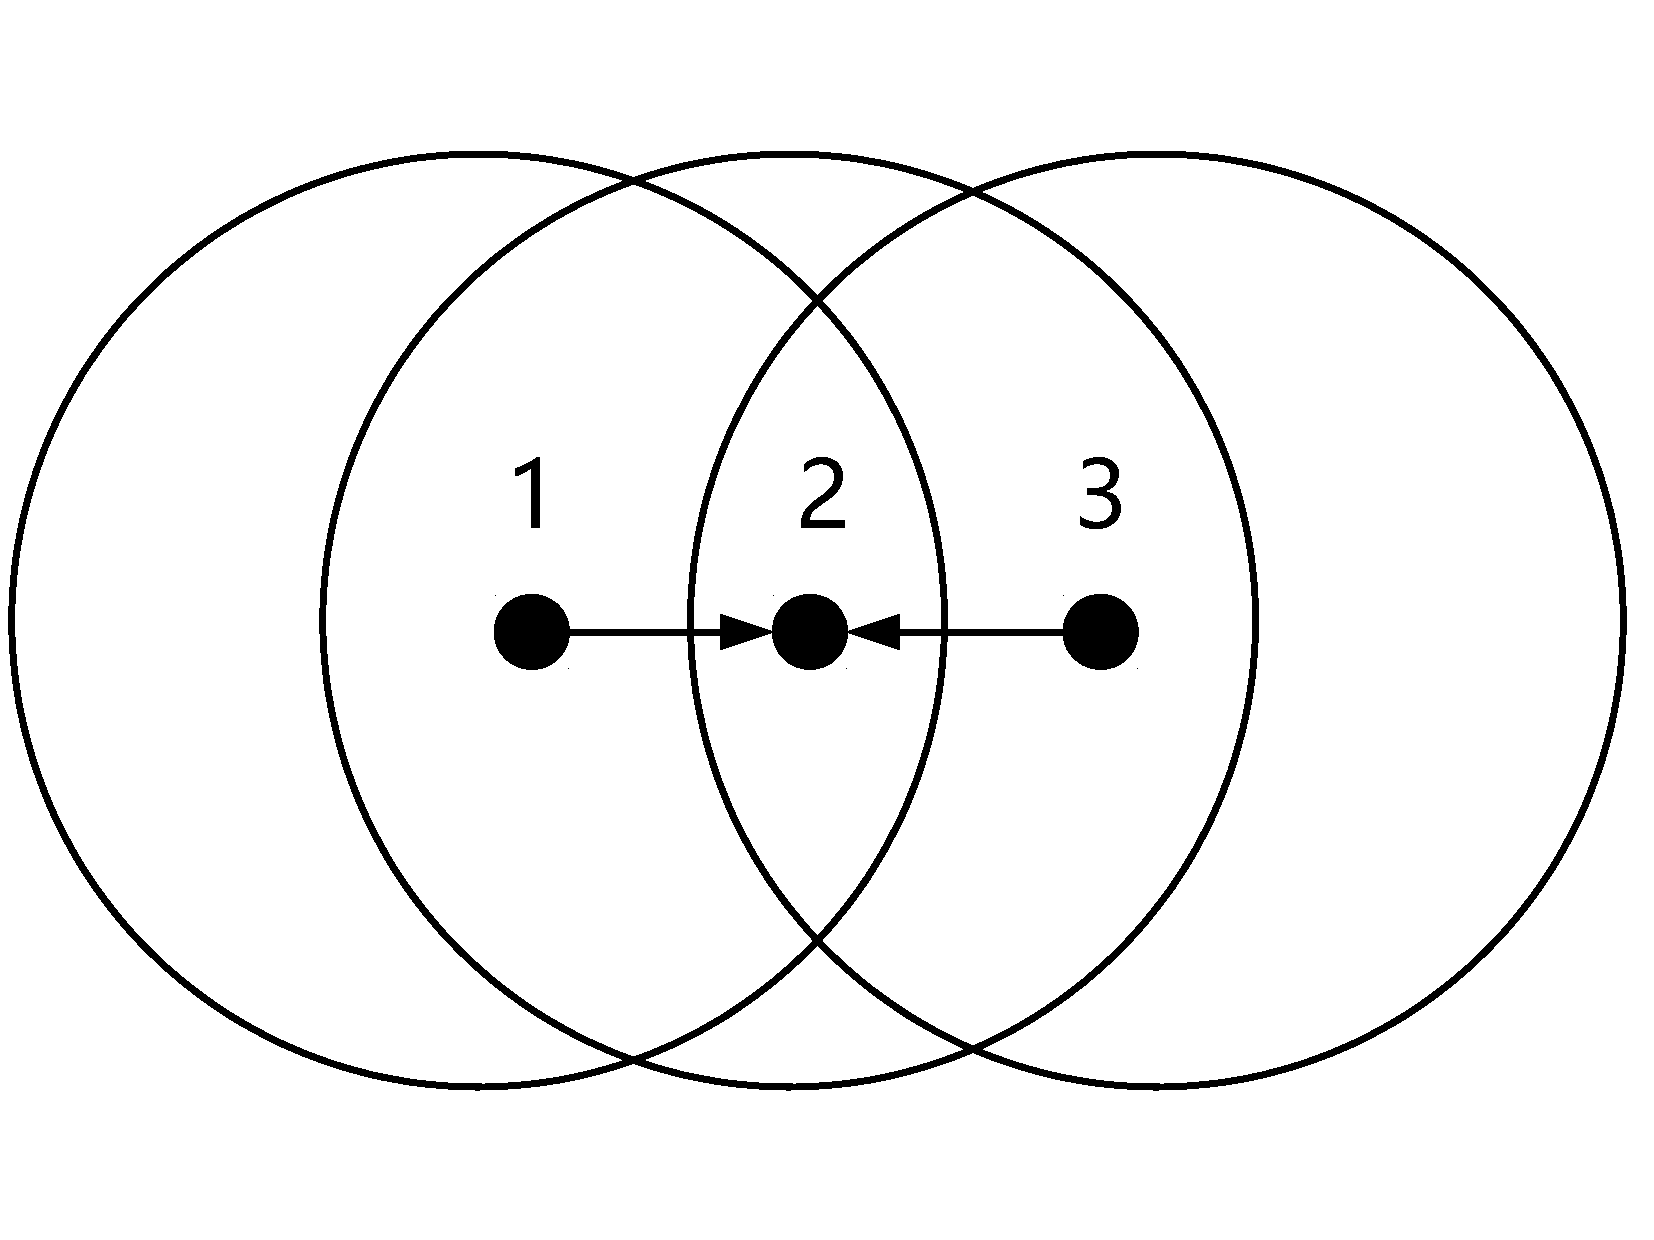
\includegraphics[scale=0.1]{figures/6.pdf}
	\caption{
		hidden terminal problem
	}
	\label{fig:example}
\end{figure}

Assuming that $P_S$ denotes the success probability of transmission. In other words, for node 1, it means the probability of no packet collision in the data interaction. Let the number of node 1's neighboring nodes be M. The hidden terminals generated by neighboring mobile nodes is Q, including $Q_s$ static terminals and $Q_m$ mobile terminals. Each hidden terminal sends data to node 1 at the rate of $\lambda$, while mobile nodeS send BCT frame at the rate of $\mu$. 

Since nodes generate data at rate of $\lambda$, $P_S$ equals the probability of neighboring nodes not generating data and hidden terminals not interfere the ongoing transmission. Thus,
\begin{equation}
P_S=\lambda(1-\lambda)^{M+Q_s}(1-\mu)^{Q_m}
\label{e1}
\end{equation}

Despite transmitting data, nodes will in the state of deferring. It will be triggered when receiving RTS frame from neighboring nodes and CTS frame from  neighboring nodes to respond hidden terminals.

The probability of receiving RTS frame is
\begin{equation}
P_{Rdefer}=(1-\lambda)\lambda M
\label{e2}
\end{equation}

The probability of receiving CTS frame is
\begin{equation}
P_{Cdefer}=(1-\lambda)\lambda Q
\label{e3}
\end{equation}

A failure period includes waiting time for sending RTS and timeout of RTS state. Let the max propagation delay be$\tau$, a failure period equals
\begin{equation}
\begin{aligned}
T_{fail}&=T_{DIFS}+Tout_{RTS}\\
&=T_{DIFS}+T_{RTS}+2\tau+T_{SIFS}+T_{CTS}
\end{aligned}
\label{e5}
\end{equation}

A success period includes RTS, CTS, DATA and ACK phases. A success period equals
\begin{equation}
\begin{aligned}
T_{suc}=&T_{DIFS}+T_{RTS}+T_{CTS}+T_{DATA}\\
&+T_{ACK}+4\tau+3T_{SIFS}
\end{aligned}
\label{e6}
\end{equation}

The deferring time caused by receiving RTS frame is
\begin{equation}
T_{Rdefer}=T_{CTS}+T_{DATA}+T_{ACK}+3\tau+3T_{SIFS}
\label{e7}
\end{equation}

The deferring time caused by receiving CTS frame is
\begin{equation}
T_{Cdefer}=T_{DATA}+T_{ACK}+2\tau+2T_{SIFS}
\label{e8}
\end{equation}

The expected time when node is busy is
\begin{equation}
\begin{aligned}
\overline B=&T_{suc}P_S+T_{fail}(\lambda-P_S )+ T_{Cdefer}P_{Cdefer}\\&+T_{Rdefer}P_{Rdefer}
\end{aligned}
\label{e9}
\end{equation}

If $ \overline B $ is greater than unit time, the node is always occupied. If $ \overline B $ is less than unit time, the remaining time equals the expection of idle time. Thus, the expected time when node is idle is
\begin{equation}
\overline I=\left\{
\begin{aligned}
1-B \ \ \ \ \ \ \ \ B<1\\
0\ \ \ \ \ \ \ \    B\ge 1
\end{aligned}
\right.
\label{e10}
\end{equation}

According to equation (\ref{11})-(\ref{e10}), the throughput of a single node can be calculated as (\ref{s1}).


\subsection {high-load transmission mode}
In the high-load transmission mode,nodes generate data at rate of $\lambda$. However, nodes generate one transmission period at rate of $\frac{\lambda}{2}$. The the success probability of transmission changes to
\begin{equation}
P_S^h=\frac{\lambda}{2}(1-\frac{\lambda}{2})^{M+Q_s}(1-\mu)^{Q_m}
\label{h1}
\end{equation}

The probability of receiving RTS frame changes to
\begin{equation}
P_{Rdefer}^h=(1-\frac{\lambda}{2})\cdot\frac{\lambda}{2} M
\end{equation}

The probability of receiving CTS frame changes to
\begin{equation}
P_{Cdefer}^h=(1-\frac{\lambda}{2})\cdot\frac{\lambda}{2} Q
\end{equation}

Since a failure period includes waiting for sending RTS and timeout of RTS state, timeout changes in the high-load transmission. As mentioned in section II, timeout of SEND state in high-load transmission mode includes one more SIFS and one more txtime of data than low-load transmission mode. A failure period changes to
\begin{equation}
\begin{aligned}
T_{fail}^h&=T_{DIFS}+Tout_{RTS}\\
&=T_{DIFS}+T_{RTS}+2\tau+T_{SIFS}+T_{CTS}
\end{aligned}
\end{equation}

A success period includes RTS, CTS, 2DATA and ACK phases. A success period changes to
\begin{equation}
\begin{aligned}
T_{suc}^h=&T_{DIFS}+T_{RTS}+T_{CTS}+2T_{DATA}\\&
+T_{ACK}+4\tau+4T_{SIFS}
\end{aligned}
\end{equation}

The deferring time caused by receiving RTS frame changes to
\begin{equation*}
T_{Rdefer}^h=T_{CTS}+2T_{DATA}+T_{ACK}+3\tau+4T_{SIFS}
\end{equation*}

The deferring time caused by receiving CTS frame changes to
\begin{equation}
T_{Cdefer}^h=2T_{DATA}+T_{ACK}+2\tau+2T_{SIFS}
\end{equation}

The expected time when node is busy equals
\begin{equation}
\begin{aligned}
\overline B^h=T_{Cdefer}^hP_{Cdefer}^h+T_{Rdefer}^hP_{Rdefer}^h
\end{aligned}
\end{equation}

The expected time when node is idle equals
\begin{equation}
\overline I^h=\left\{
\begin{aligned}
1-\overline B^h \ \ \ \ \ \ \ \ B<1\\
0\ \ \ \ \ \ \ \    B\ge 1
\end{aligned}
\right.
\label{h2}
\end{equation}

According to equation (\ref{11}) and (\ref{h1})-(\ref{h2}), the throughput of a single node in high-load transmission mode can be calculated as equation (\ref{s2}).

\newcounter{mytempeqncnt}

\begin{figure*}[!h]
	
	\normalsize
	
	\setcounter{mytempeqncnt}{\value{equation}}
	
	%\setcounter{equation}{5}
	
	\begin{equation}
	\begin{aligned}
	S&=\frac{\overline U}{\overline B+\overline I}\\&=\frac{T_{DATA}}{ T_{suc}P_S+T_{fail}(\lambda-P_S )+ T_{Cdefer}P_{Cdefer}+T_{Rdefer}P_{Rdefer}+\overline I}
	\end{aligned}
	\label{s1}
	\end{equation}
	
	\begin{equation}
	\begin{aligned}
	S^h&=\frac{\overline U^h}{\overline B^h+\overline I^h}\\&=\frac{2T_{DATA}}{ T_{suc}^h P_S^h+T_{fail}^h(\frac{\lambda}{2}-P_S^h )+ T_{Cdefer}^hP_{Cdefer}^h+T_{Rdefer}^hP_{Rdefer}^h+\overline I^h}
	\end{aligned}
	\label{s2}
	\end{equation}
	\setcounter{equation}{\value{mytempeqncnt}}
	
	\hrulefill
	
	\vspace*{4pt}
	
\end{figure*}

\section{simulation result}

In this section, we evaluate the performance of LACC-M in the aspects of throughput, average end-to-end delay, successful delivery rate and average energy consumption using Aqua-Sim\cite{xie2009aqua}. 

We also make performance comparisons with two contention-based protocols, SFAMA\cite{molins2007slotted} and UWALOHA\cite{de2011characterization}. Results show that LACC-M achieves a good performance in designated scenarios.

\subsection{scenario with two mobile nodes}
The protocol is designed for the scenario that mobile nodes collect data from static nodes in single-hop comunication. The simulation scenario is set as fig.\ref{2scen}. There are twelve static black nodes deployed underwater, two mobile red nodes moving at rate of 2.5 m/s. The distance between adjacent static nodes is 2000m. The size of a packet is 300 Bytes.

\begin{figure}[!h]
	\centering
	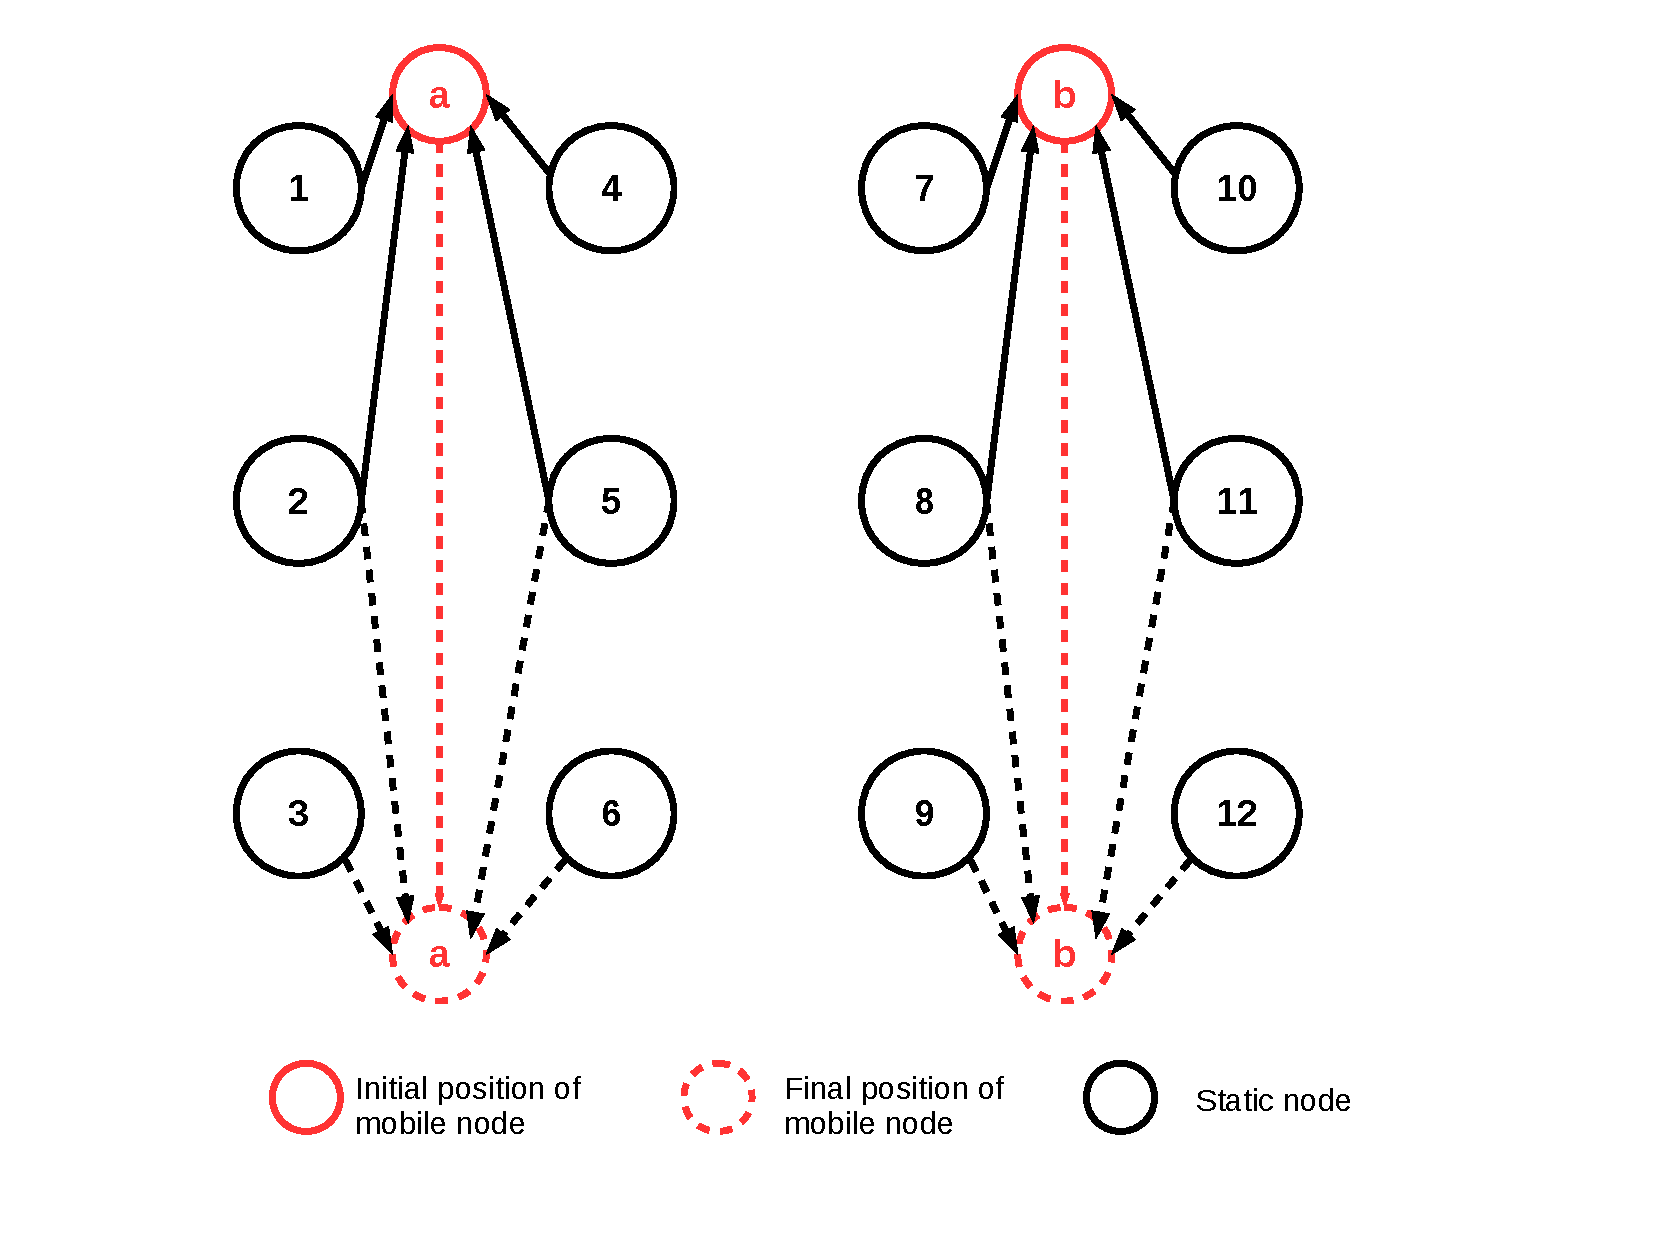
\includegraphics[scale=0.25]{figures/2scen.pdf}
	\caption{
		scenario with two mobile nodes
	}
	\label{2scen}
\end{figure}

The parameter of communication modem makes reference to Evologics S2CR 18/34 modem. Transmission range is set 3000m. Working frequency is 10khz and transmission rate is 1kbps. Power settings are 30 W for transmission, 1 W for reception, and 0.2 W for idle state.


Using the equation (\ref{s1}) and (\ref{s2}), we can evaluate the performance of LACC-M in theory. According to the number of neighboring nodes and hidden terminals, the whole simulation time of one node should be divided into different time periods. The throughput of 12 static nodes in all time periods is accumulated and then theoretical throughput of the network is obtained.

We take 30 data generating rate from 0 to 0.36pkt/s (total generating packets of 12 nodes) as the x-axis to obtain the throughput curve. The result takes average of 30 times of simulations.

As shown in fig. \ref{theory}, the theoretical curve is consistent with the trend of the simulated curve. Errors between them is acceptable and mainly come from the simplification of the performance analysis.

\begin{figure}[!h]
	\centering
	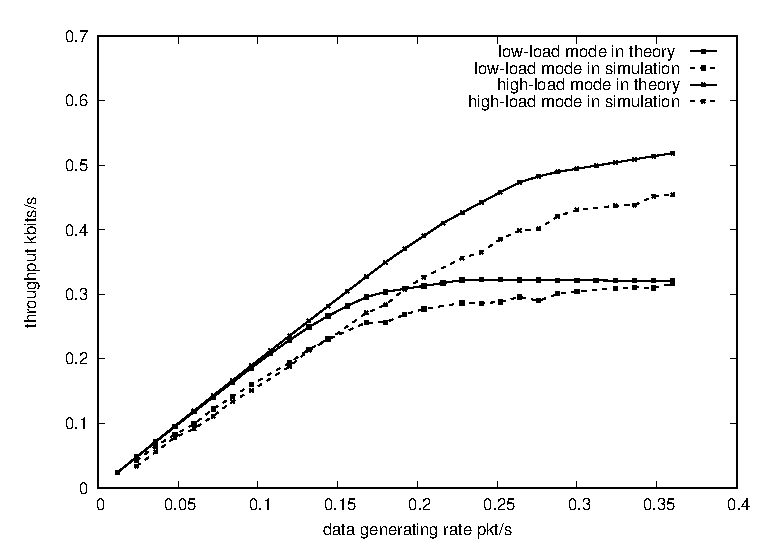
\includegraphics[scale=0.6]{figures/lilun.eps}
	\caption{
		theoretical and simulated throughput
	}
	\label{theory}
\end{figure}

Fig.\ref{fig:1} displays the performance comparisons of three MAC protocols, LACC-M, SFAMA and UWALOHA. LACC-M's performance in low-load and high-load transmission modes are also attached to show the differences of two modes.
\begin{figure*}[!h]
	\centering                                                     \subfigure[performance comparison of throughput]
	{                    \begin{minipage}{7cm}\centering                                      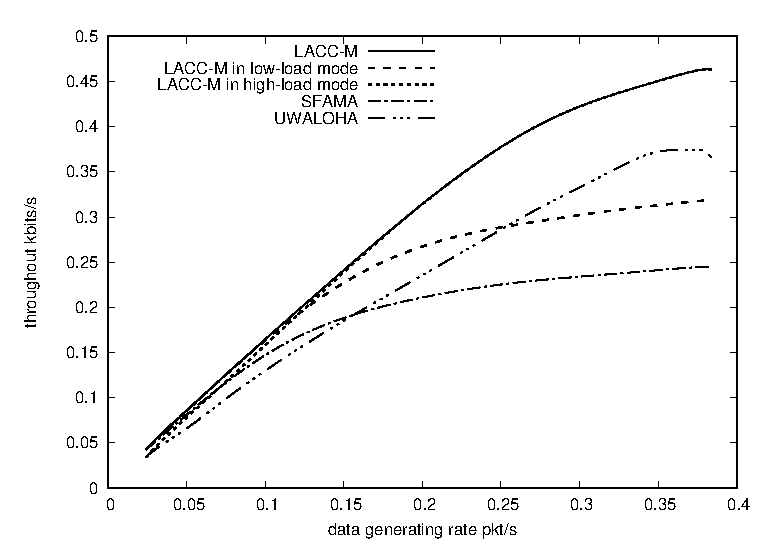
\includegraphics[scale=0.5]{figures/2nodea.eps} 
	\label{21}
	\end{minipage}
	}
	\subfigure[performance comparison of average end-to-end delay]
	{                    \begin{minipage}{7cm}\centering                                      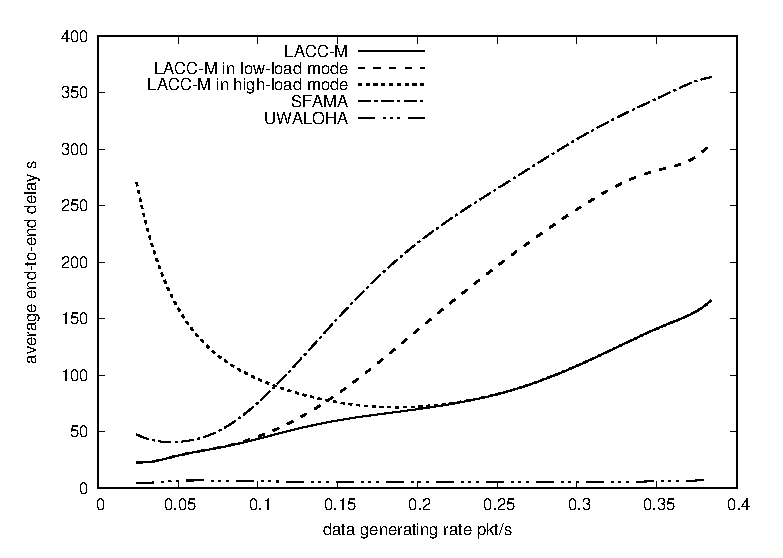
\includegraphics[scale=0.5]{figures/2nodeb.eps}    
	\label{22}            
	\end{minipage}
	}
	\subfigure[performance comparison of successful delivery rate]
	{                    \begin{minipage}{7cm}\centering                                      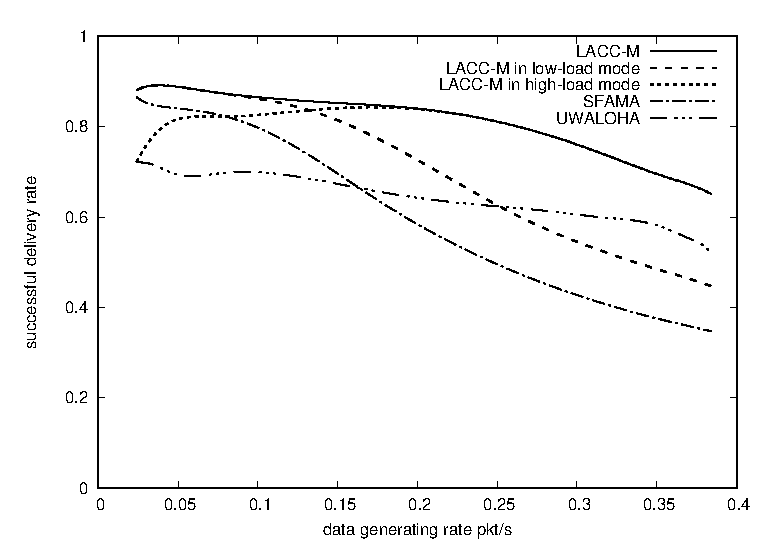
\includegraphics[scale=0.5]{figures/2nodec.eps} 
	\label{23}
	\end{minipage}
	}
	\subfigure[performance comparison of average comsumption]
	{                 \begin{minipage}{7cm}\centering                                      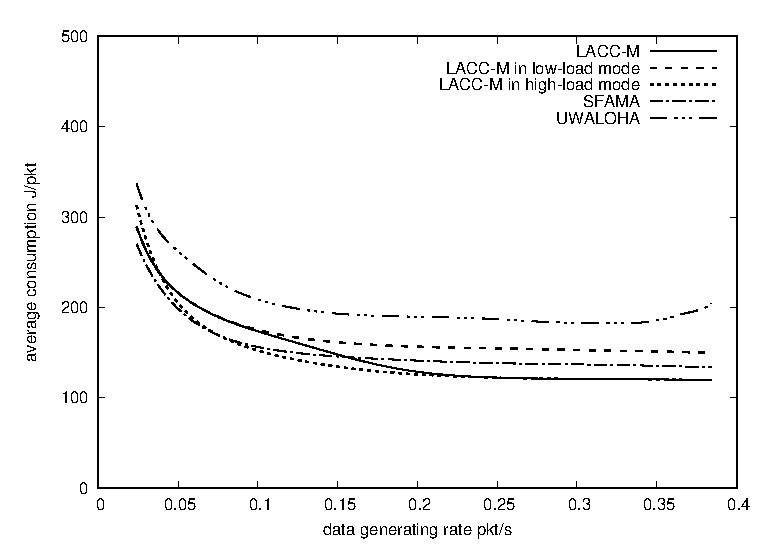
\includegraphics[scale=0.5]{figures/2noded.eps} 
	\label{24}
	\end{minipage}
	}
					
	\caption{performance comparisons with two mobile nodes}    
    \label{fig:1}                                                 
\end{figure*}
				
We observe that the throughput of three MAC protocols increases along with the traffic load, while the growth rate declines in fig.\ref{21}. The average end-to-end delay is steadily advancing with the increase of data generating rate in fig.\ref{22}. The successful delivery rate and energy consumption decrease as the traffic load grows in fig.\ref{23} and in fig.\ref{24}.

When the data generating rate is relatively high, high-load transmission mode outperforms other protocols in aspects of throughput, successful delivery rate and energy consumption. This is because the cost of handshake mechanism is expensive when the traffic load is high.

At the same time, high-load transmission mode owns higher average end-to-end delay, larger energy consumption and lower successful delivery rate when the data generating rate is relatively low. The reason is that transmitting two data frames at one time brings less transmission and longer waiting time.

It proves that specific transmission modes for different loads is necessary and effective. Meanwhile, in the single-hop data-collection scene, the mobile nodes are able to tell the load states of the network and choose corresponding modes.

As for UWALOH, the energy consumption is quiet high because the retransmission of data frames consumes great quantity of energy in fig.\ref{24}. As for SFAMA, it behaves mediocrely when the traffic load is high.


\subsection{scenario with three mobile nodes}
In order of simulating the circumstance that one static node senses multiple mobile nodes at one time, we add one mobile node in the network. The scenario is shown in fig.\ref{3scen}. Parameter settings of this simulation is similar to the first one. 

 \begin{figure}[!h]
 	\centering
 	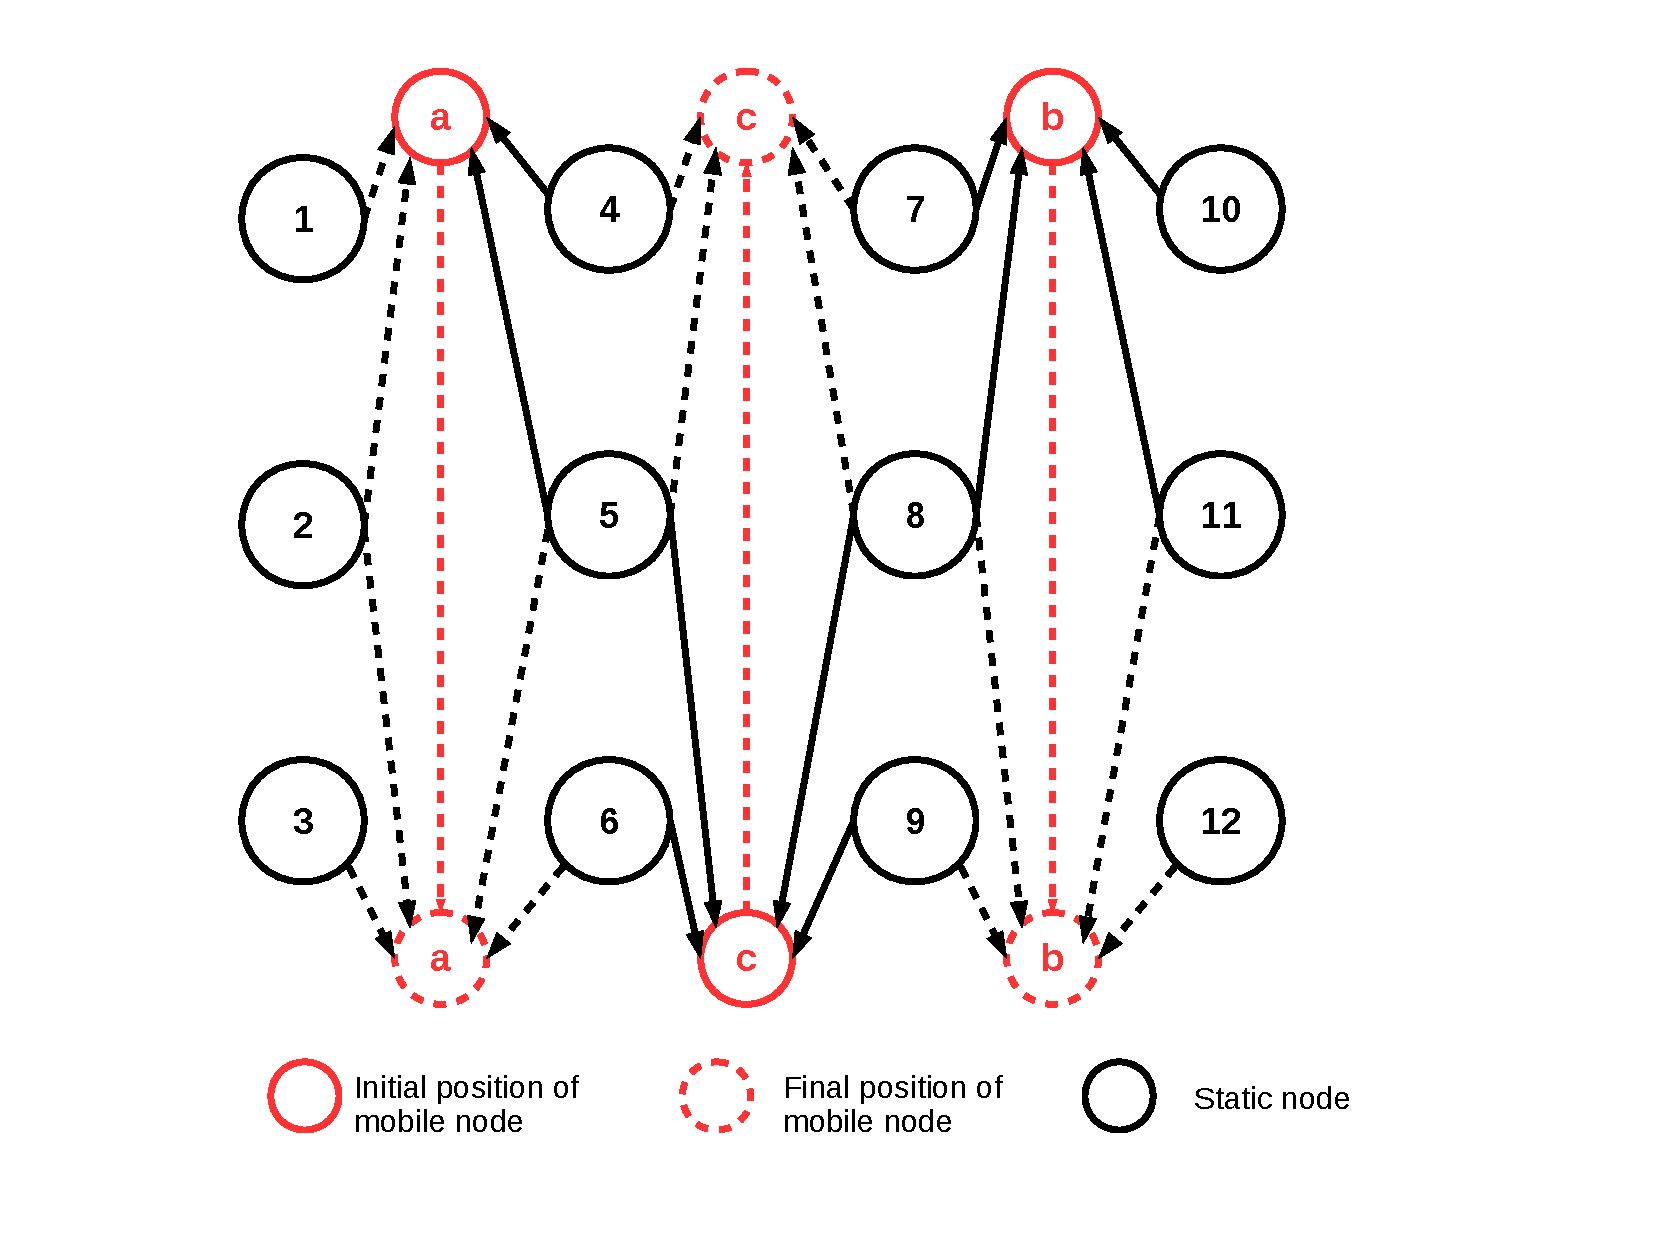
\includegraphics[scale=0.25]{figures/3scen.pdf}
 	\caption{
 		scenario with three mobile nodes
 	}
 	\label{3scen}
 \end{figure}

Fig.\ref{fig:2} exhibits the results. The general trend of the performance of throughput, average end-to-end delay, successful delivery rate and energy transmission is consistent with the last simulation.

The addition of the mobile node makes the network topology more dynamic. Thus, in fig.\ref{31},the throughput of the high load network is lower than that of the scenario with two mobile nodes. The critical value of the network is also reduced.

Since the load of the network does not change, the load of a single mobile node is reduced. The optimization brought by high-load transmission mode becomes less obvious compared with that of two mobile nodes.

The utilization ratio of the channel is improved with the addition of the mobile node, so the successful delivery rate is higher in fig.\ref{33}. However, the new mobile node also brings more collisions. Therefore, compared with the network of two mobile nodes, the proposed LACC-M protocol is more sensitive to changes of network load.

\begin{figure*}[!h]
	\centering                                                     \subfigure[performance comparison of throughput]
	{                    \begin{minipage}{7cm}\centering                                      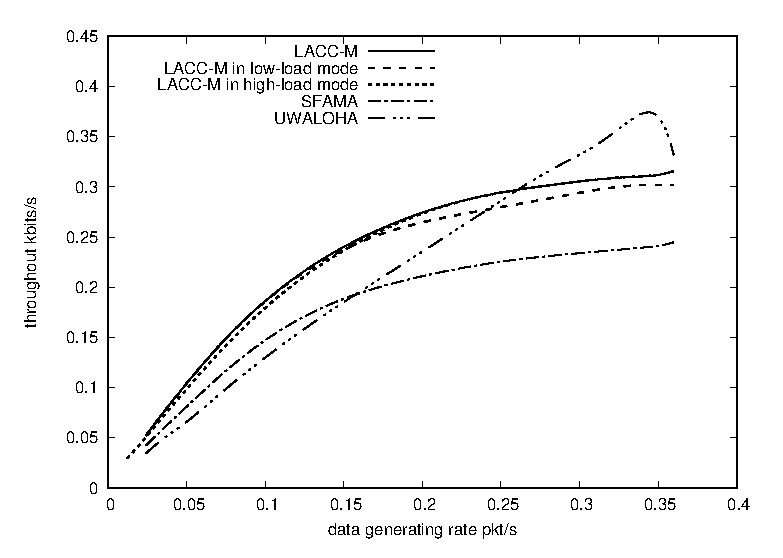
\includegraphics[scale=0.5]{figures/3nodea.eps} 
	\label{31} 
	\end{minipage}
	}
	\subfigure[performance comparison of average end-to-end delay]
	{                    \begin{minipage}{7cm}\centering                                      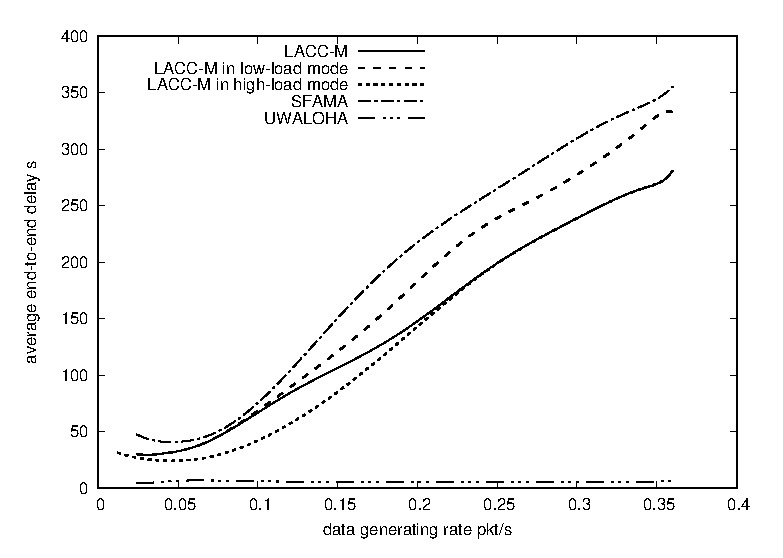
\includegraphics[scale=0.5]{figures/3nodeb.eps}
	\label{32}                
	\end{minipage}
	}
	\subfigure[performance comparison of successful delivery rate]
	{                    \begin{minipage}{7cm}\centering                                      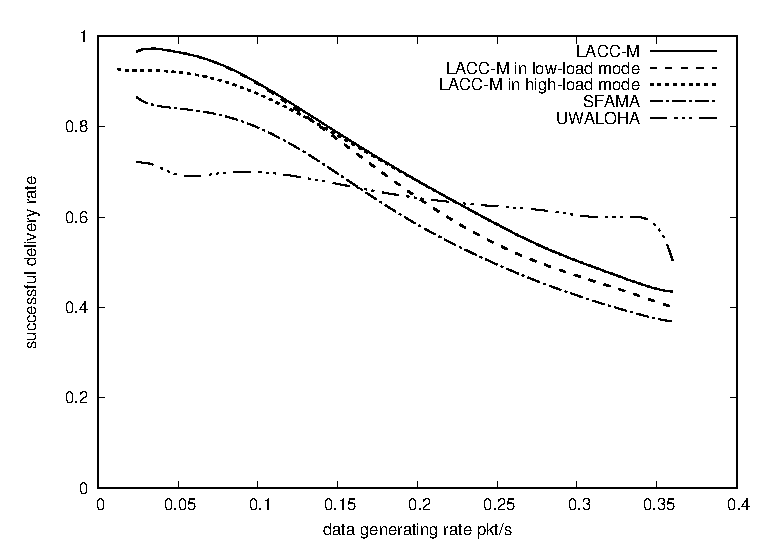
\includegraphics[scale=0.5]{figures/3nodec.eps} 
	\label{33}
	\end{minipage}
	}
	\subfigure[performance comparison of average comsumption]
	{                 \begin{minipage}{7cm}\centering                                      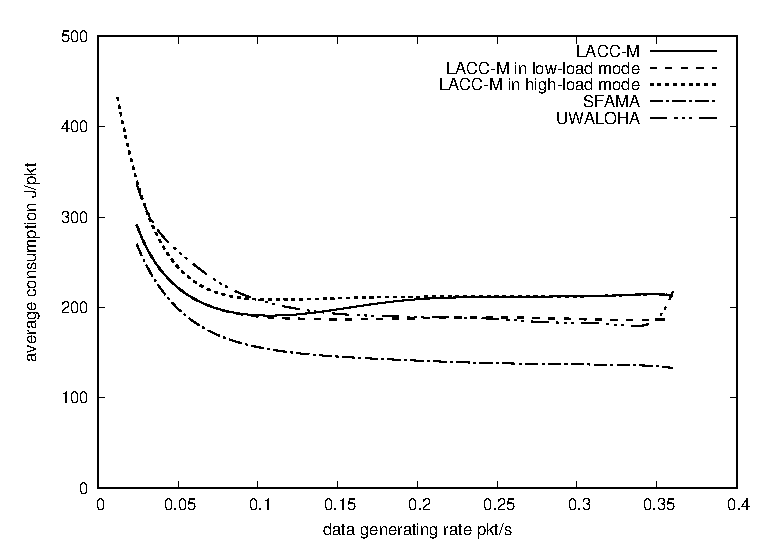
\includegraphics[scale=0.5]{figures/3noded.eps} 
	\label{34}
	\end{minipage}
	}
	
	\caption{performance comparisons with three mobile nodes}    
    \label{fig:2}                                                 
\end{figure*}                                                 

\section{conclusion and future work}
In this paper, we propose a load adaptive CSMA/CA MAC for mobile underwater acoustic network, LACC-M. The protocol is designed for the scenario that mobile nodes like UUVs/AUVs tour around the area of pre-deployed static nodes and gather data from static nodes. BCT frame is introduced to allow the mobile nodes access and exit the network as soon as possible without interfering the ongoing
transmission. Different transmission modes are applied depending on different network loads. Simulations show that LACC-M has higher
throughput, smaller end-to-end delay, acceptable successful delivery rate, and better energy consumption compared with two other contention-based protocol, SFAMA and UWALOHA. It has high tolerance of different network loads in the pre-set occasions.

There remains something to be studied. LACC-M is
presented for the single-hop scenario. How to evaluate the network load in the multi-hop scenario and decrease the energy consumption brought by multiple sendings need to be contemplated.

\bibliographystyle{IEEEtran}
\bibliography{IEEEexample,reference}
\end{document}
